% !TeX program = pdflatex
% !TeX root = FCGraphCuttableQ.tex

\documentclass[../FeynCalcManual.tex]{subfiles}
\begin{document}
\hypertarget{fcgraphcuttableq}{
\section{FCGraphCuttableQ}\label{fcgraphcuttableq}\index{FCGraphCuttableQ}}

\texttt{FCGraphCuttableQ[\allowbreak{}\{\allowbreak{}edges,\ \allowbreak{}labels\},\ \allowbreak{}\{\allowbreak{}m1,\ \allowbreak{}m2,\ \allowbreak{}...\}]}
checks whether the given graph representing a loop integral can be cut
such, that no propagator containing masses
\texttt{\{\allowbreak{}m1,\ \allowbreak{}m2,\ \allowbreak{}...\}} goes
on shell. To that aim \texttt{labels} must contain masses occurring in
the respective propagators.

\texttt{FCGraphCuttableQ} uses \texttt{FCGraphFindPath} as the back-end.

The list \texttt{\{\allowbreak{}edges,\ \allowbreak{}labels\}} can be
the output of \texttt{FCLoopIntegralToGraph}.

\subsection{See also}

\hyperlink{toc}{Overview}, \hyperlink{fcgraphfindpath}{FCGraphFindPath},
\hyperlink{fcloopintegraltograph}{FCLoopIntegralToGraph},
\hyperlink{samesideexternaledges}{SameSideExternalEdges}.

\subsection{Examples}

This integral has no imaginary part due to the massive \texttt{m1}-line
that cannot be cut

\begin{Shaded}
\begin{Highlighting}[]
\NormalTok{graph1 }\ExtensionTok{=} \OperatorTok{\{\{}\SpecialCharTok{{-}}\DecValTok{3} \OtherTok{{-}\textgreater{}} \DecValTok{2}\OperatorTok{,} \SpecialCharTok{{-}}\DecValTok{1} \OtherTok{{-}\textgreater{}} \DecValTok{1}\OperatorTok{,} \DecValTok{1} \OtherTok{{-}\textgreater{}} \DecValTok{3}\OperatorTok{,} \DecValTok{1} \OtherTok{{-}\textgreater{}} \DecValTok{4}\OperatorTok{,} \DecValTok{2} \OtherTok{{-}\textgreater{}} \DecValTok{3}\OperatorTok{,} \DecValTok{2} \OtherTok{{-}\textgreater{}} \DecValTok{4}\OperatorTok{,} \DecValTok{2} \OtherTok{{-}\textgreater{}} \DecValTok{4}\OperatorTok{,} \DecValTok{3} \OtherTok{{-}\textgreater{}} \DecValTok{4}\OperatorTok{\},} \OperatorTok{\{}\NormalTok{q1}\OperatorTok{,}\NormalTok{ q1}\OperatorTok{,} \OperatorTok{\{}\NormalTok{p3}\OperatorTok{,} \DecValTok{1}\OperatorTok{,}\NormalTok{ m1}\SpecialCharTok{\^{}}\DecValTok{2}\OperatorTok{\},} \OperatorTok{\{}\NormalTok{p3 }\SpecialCharTok{+}\NormalTok{ q1}\OperatorTok{,} \DecValTok{1}\OperatorTok{,}\NormalTok{ m1}\SpecialCharTok{\^{}}\DecValTok{2}\OperatorTok{\},} 
     \OperatorTok{\{}\NormalTok{p2}\OperatorTok{,} \DecValTok{1}\OperatorTok{,}\NormalTok{ m1}\SpecialCharTok{\^{}}\DecValTok{2}\OperatorTok{\},} \OperatorTok{\{}\NormalTok{p1 }\SpecialCharTok{+}\NormalTok{ q1}\OperatorTok{,} \DecValTok{1}\OperatorTok{,}\NormalTok{ m2}\SpecialCharTok{\^{}}\DecValTok{2}\OperatorTok{\},} \OperatorTok{\{}\NormalTok{p1 }\SpecialCharTok{{-}}\NormalTok{ p2}\OperatorTok{,} \DecValTok{1}\OperatorTok{,}\NormalTok{ m1}\SpecialCharTok{\^{}}\DecValTok{2}\OperatorTok{\},} \OperatorTok{\{}\NormalTok{p2 }\SpecialCharTok{{-}}\NormalTok{ p3}\OperatorTok{,} \DecValTok{1}\OperatorTok{,} \DecValTok{0}\OperatorTok{\}\},} \OperatorTok{\{}\DecValTok{0}\OperatorTok{,} \DecValTok{0}\OperatorTok{,}\NormalTok{ SFAD}\OperatorTok{[\{\{}\FunctionTok{I}\SpecialCharTok{*}\NormalTok{p3}\OperatorTok{,} \DecValTok{0}\OperatorTok{\},} \OperatorTok{\{}\SpecialCharTok{{-}}\NormalTok{m1}\SpecialCharTok{\^{}}\DecValTok{2}\OperatorTok{,} \SpecialCharTok{{-}}\DecValTok{1}\OperatorTok{\},} \DecValTok{1}\OperatorTok{\}],} 
\NormalTok{     SFAD}\OperatorTok{[\{\{}\FunctionTok{I}\SpecialCharTok{*}\NormalTok{p2}\OperatorTok{,} \DecValTok{0}\OperatorTok{\},} \OperatorTok{\{}\SpecialCharTok{{-}}\NormalTok{m1}\SpecialCharTok{\^{}}\DecValTok{2}\OperatorTok{,} \SpecialCharTok{{-}}\DecValTok{1}\OperatorTok{\},} \DecValTok{1}\OperatorTok{\}],}\NormalTok{ SFAD}\OperatorTok{[\{\{}\FunctionTok{I}\SpecialCharTok{*}\NormalTok{(p3 }\SpecialCharTok{+}\NormalTok{ q1)}\OperatorTok{,} \DecValTok{0}\OperatorTok{\},} \OperatorTok{\{}\SpecialCharTok{{-}}\NormalTok{m1}\SpecialCharTok{\^{}}\DecValTok{2}\OperatorTok{,} \SpecialCharTok{{-}}\DecValTok{1}\OperatorTok{\},} \DecValTok{1}\OperatorTok{\}],}\NormalTok{ SFAD}\OperatorTok{[\{\{}\FunctionTok{I}\SpecialCharTok{*}\NormalTok{(p1 }\SpecialCharTok{+}\NormalTok{ q1)}\OperatorTok{,} \DecValTok{0}\OperatorTok{\},} 
       \OperatorTok{\{}\SpecialCharTok{{-}}\NormalTok{m2}\SpecialCharTok{\^{}}\DecValTok{2}\OperatorTok{,} \SpecialCharTok{{-}}\DecValTok{1}\OperatorTok{\},} \DecValTok{1}\OperatorTok{\}],}\NormalTok{ SFAD}\OperatorTok{[\{\{}\FunctionTok{I}\SpecialCharTok{*}\NormalTok{(p2 }\SpecialCharTok{{-}}\NormalTok{ p3)}\OperatorTok{,} \DecValTok{0}\OperatorTok{\},} \OperatorTok{\{}\DecValTok{0}\OperatorTok{,} \SpecialCharTok{{-}}\DecValTok{1}\OperatorTok{\},} \DecValTok{1}\OperatorTok{\}],}\NormalTok{ SFAD}\OperatorTok{[\{\{}\FunctionTok{I}\SpecialCharTok{*}\NormalTok{(p1 }\SpecialCharTok{{-}}\NormalTok{ p2)}\OperatorTok{,} \DecValTok{0}\OperatorTok{\},} \OperatorTok{\{}\SpecialCharTok{{-}}\NormalTok{m1}\SpecialCharTok{\^{}}\DecValTok{2}\OperatorTok{,} \SpecialCharTok{{-}}\DecValTok{1}\OperatorTok{\},} \DecValTok{1}\OperatorTok{\}]\},} \DecValTok{1}\OperatorTok{\}}\NormalTok{;}
\end{Highlighting}
\end{Shaded}

\begin{Shaded}
\begin{Highlighting}[]
\NormalTok{FCLoopGraphPlot}\OperatorTok{[}\NormalTok{graph1}\OperatorTok{,} \FunctionTok{GraphPlot} \OtherTok{{-}\textgreater{}} \OperatorTok{\{}\FunctionTok{MultiedgeStyle} \OtherTok{{-}\textgreater{}} \FloatTok{0.35}\OperatorTok{,} \FunctionTok{Frame} \OtherTok{{-}\textgreater{}} \ConstantTok{True}\OperatorTok{\},} \FunctionTok{Style} \OtherTok{{-}\textgreater{}} \OperatorTok{\{}
    \OperatorTok{\{}\StringTok{"InternalLine"}\OperatorTok{,}\NormalTok{ \_}\OperatorTok{,}\NormalTok{ \_}\OperatorTok{,} \AttributeTok{mm\_} \SpecialCharTok{/}\NormalTok{; ! }\FunctionTok{FreeQ}\OperatorTok{[}\NormalTok{mm}\OperatorTok{,}\NormalTok{ mg }\SpecialCharTok{|}\NormalTok{ m3}\OperatorTok{]\}} \OtherTok{{-}\textgreater{}} \OperatorTok{\{}\FunctionTok{Red}\OperatorTok{,} \FunctionTok{Thick}\OperatorTok{,} \FunctionTok{Dashed}\OperatorTok{\},} 
    \OperatorTok{\{}\StringTok{"InternalLine"}\OperatorTok{,}\NormalTok{ \_}\OperatorTok{,}\NormalTok{ \_}\OperatorTok{,} \AttributeTok{mm\_} \SpecialCharTok{/}\NormalTok{; ! }\FunctionTok{FreeQ}\OperatorTok{[}\NormalTok{mm}\OperatorTok{,}\NormalTok{ mc }\SpecialCharTok{|}\NormalTok{ m2}\OperatorTok{]\}} \OtherTok{{-}\textgreater{}} \OperatorTok{\{}\FunctionTok{Blue}\OperatorTok{,} \FunctionTok{Thick}\OperatorTok{,} \FunctionTok{Dashed}\OperatorTok{\},} 
    \OperatorTok{\{}\StringTok{"InternalLine"}\OperatorTok{,}\NormalTok{ \_}\OperatorTok{,}\NormalTok{ \_}\OperatorTok{,} \AttributeTok{mm\_} \SpecialCharTok{/}\NormalTok{; ! }\FunctionTok{FreeQ}\OperatorTok{[}\NormalTok{mm}\OperatorTok{,}\NormalTok{ mb }\SpecialCharTok{|}\NormalTok{ m1}\OperatorTok{]\}} \OtherTok{{-}\textgreater{}} \OperatorTok{\{}\FunctionTok{Black}\OperatorTok{,} \FunctionTok{Thick}\OperatorTok{\}} 
   \OperatorTok{\}]}
\end{Highlighting}
\end{Shaded}

\FloatBarrier
\begin{figure}[!ht]
\centering
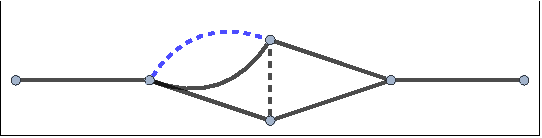
\includegraphics[width=0.6\linewidth]{img/11ouyv2qtno96.pdf}
\end{figure}
\FloatBarrier

\begin{Shaded}
\begin{Highlighting}[]
\NormalTok{FCGraphCuttableQ}\OperatorTok{[}\NormalTok{graph1}\OperatorTok{,} \OperatorTok{\{}\NormalTok{m1}\OperatorTok{\}]}
\end{Highlighting}
\end{Shaded}

\begin{dmath*}\breakingcomma
\text{False}
\end{dmath*}

\begin{Shaded}
\begin{Highlighting}[]
\NormalTok{graph2 }\ExtensionTok{=} \OperatorTok{\{\{}\SpecialCharTok{{-}}\DecValTok{3} \OtherTok{{-}\textgreater{}} \DecValTok{2}\OperatorTok{,} \SpecialCharTok{{-}}\DecValTok{1} \OtherTok{{-}\textgreater{}} \DecValTok{1}\OperatorTok{,} \DecValTok{1} \OtherTok{{-}\textgreater{}} \DecValTok{3}\OperatorTok{,} \DecValTok{1} \OtherTok{{-}\textgreater{}} \DecValTok{4}\OperatorTok{,} \DecValTok{2} \OtherTok{{-}\textgreater{}} \DecValTok{4}\OperatorTok{,} \DecValTok{2} \OtherTok{{-}\textgreater{}} \DecValTok{5}\OperatorTok{,} \DecValTok{3} \OtherTok{{-}\textgreater{}} \DecValTok{5}\OperatorTok{,} \DecValTok{3} \OtherTok{{-}\textgreater{}} \DecValTok{6}\OperatorTok{,} \DecValTok{4} \OtherTok{{-}\textgreater{}} \DecValTok{6}\OperatorTok{,} \DecValTok{5} \OtherTok{{-}\textgreater{}} \DecValTok{6}\OperatorTok{\},} \OperatorTok{\{}\NormalTok{q1}\OperatorTok{,}\NormalTok{ q1}\OperatorTok{,} \OperatorTok{\{}\NormalTok{p3}\OperatorTok{,} \DecValTok{1}\OperatorTok{,} \DecValTok{0}\OperatorTok{\},} \OperatorTok{\{}\NormalTok{p3 }\SpecialCharTok{+}\NormalTok{ q1}\OperatorTok{,} \DecValTok{1}\OperatorTok{,}\NormalTok{ m1}\SpecialCharTok{\^{}}\DecValTok{2}\OperatorTok{\},} 
     \OperatorTok{\{}\NormalTok{p1 }\SpecialCharTok{+}\NormalTok{ q1}\OperatorTok{,} \DecValTok{1}\OperatorTok{,} \DecValTok{0}\OperatorTok{\},} \OperatorTok{\{}\NormalTok{p1}\OperatorTok{,} \DecValTok{1}\OperatorTok{,}\NormalTok{ m1}\SpecialCharTok{\^{}}\DecValTok{2}\OperatorTok{\},} \OperatorTok{\{}\NormalTok{p2}\OperatorTok{,} \DecValTok{1}\OperatorTok{,}\NormalTok{ m1}\SpecialCharTok{\^{}}\DecValTok{2}\OperatorTok{\},} \OperatorTok{\{}\NormalTok{p2 }\SpecialCharTok{{-}}\NormalTok{ p3}\OperatorTok{,} \DecValTok{1}\OperatorTok{,}\NormalTok{ m1}\SpecialCharTok{\^{}}\DecValTok{5}\OperatorTok{\},} \OperatorTok{\{}\SpecialCharTok{{-}}\NormalTok{p1 }\SpecialCharTok{+}\NormalTok{ p3}\OperatorTok{,} \DecValTok{1}\OperatorTok{,}\NormalTok{ m2}\SpecialCharTok{\^{}}\DecValTok{2}\OperatorTok{\},} \OperatorTok{\{}\NormalTok{p1 }\SpecialCharTok{{-}}\NormalTok{ p2}\OperatorTok{,} \DecValTok{1}\OperatorTok{,}\NormalTok{ m1}\SpecialCharTok{\^{}}\DecValTok{2}\OperatorTok{\}\},} 
    \OperatorTok{\{}\DecValTok{0}\OperatorTok{,} \DecValTok{0}\OperatorTok{,}\NormalTok{ SFAD}\OperatorTok{[\{\{}\FunctionTok{I}\SpecialCharTok{*}\NormalTok{p3}\OperatorTok{,} \DecValTok{0}\OperatorTok{\},} \OperatorTok{\{}\DecValTok{0}\OperatorTok{,} \SpecialCharTok{{-}}\DecValTok{1}\OperatorTok{\},} \DecValTok{1}\OperatorTok{\}],}\NormalTok{ SFAD}\OperatorTok{[\{\{}\FunctionTok{I}\SpecialCharTok{*}\NormalTok{(p1 }\SpecialCharTok{+}\NormalTok{ q1)}\OperatorTok{,} \DecValTok{0}\OperatorTok{\},} \OperatorTok{\{}\DecValTok{0}\OperatorTok{,} \SpecialCharTok{{-}}\DecValTok{1}\OperatorTok{\},} \DecValTok{1}\OperatorTok{\}],}\NormalTok{ SFAD}\OperatorTok{[\{\{}\FunctionTok{I}\SpecialCharTok{*}\NormalTok{p2}\OperatorTok{,} \DecValTok{0}\OperatorTok{\},} 
       \OperatorTok{\{}\SpecialCharTok{{-}}\NormalTok{m1}\SpecialCharTok{\^{}}\DecValTok{2}\OperatorTok{,} \SpecialCharTok{{-}}\DecValTok{1}\OperatorTok{\},} \DecValTok{1}\OperatorTok{\}],}\NormalTok{ SFAD}\OperatorTok{[\{\{}\FunctionTok{I}\SpecialCharTok{*}\NormalTok{p1}\OperatorTok{,} \DecValTok{0}\OperatorTok{\},} \OperatorTok{\{}\SpecialCharTok{{-}}\NormalTok{m1}\SpecialCharTok{\^{}}\DecValTok{2}\OperatorTok{,} \SpecialCharTok{{-}}\DecValTok{1}\OperatorTok{\},} \DecValTok{1}\OperatorTok{\}],}\NormalTok{ SFAD}\OperatorTok{[\{\{}\FunctionTok{I}\SpecialCharTok{*}\NormalTok{(p3 }\SpecialCharTok{+}\NormalTok{ q1)}\OperatorTok{,} \DecValTok{0}\OperatorTok{\},} \OperatorTok{\{}\SpecialCharTok{{-}}\NormalTok{m1}\SpecialCharTok{\^{}}\DecValTok{2}\OperatorTok{,} \SpecialCharTok{{-}}\DecValTok{1}\OperatorTok{\},} \DecValTok{1}\OperatorTok{\}],} 
\NormalTok{     SFAD}\OperatorTok{[\{\{}\FunctionTok{I}\SpecialCharTok{*}\NormalTok{(}\SpecialCharTok{{-}}\NormalTok{p1 }\SpecialCharTok{+}\NormalTok{ p3)}\OperatorTok{,} \DecValTok{0}\OperatorTok{\},} \OperatorTok{\{}\SpecialCharTok{{-}}\NormalTok{m2}\SpecialCharTok{\^{}}\DecValTok{2}\OperatorTok{,} \SpecialCharTok{{-}}\DecValTok{1}\OperatorTok{\},} \DecValTok{1}\OperatorTok{\}],}\NormalTok{ SFAD}\OperatorTok{[\{\{}\FunctionTok{I}\SpecialCharTok{*}\NormalTok{(p2 }\SpecialCharTok{{-}}\NormalTok{ p3)}\OperatorTok{,} \DecValTok{0}\OperatorTok{\},} \OperatorTok{\{}\SpecialCharTok{{-}}\NormalTok{m1}\SpecialCharTok{\^{}}\DecValTok{5}\OperatorTok{,} \SpecialCharTok{{-}}\DecValTok{1}\OperatorTok{\},} \DecValTok{1}\OperatorTok{\}],} 
\NormalTok{     SFAD}\OperatorTok{[\{\{}\FunctionTok{I}\SpecialCharTok{*}\NormalTok{(p1 }\SpecialCharTok{{-}}\NormalTok{ p2)}\OperatorTok{,} \DecValTok{0}\OperatorTok{\},} \OperatorTok{\{}\SpecialCharTok{{-}}\NormalTok{m1}\SpecialCharTok{\^{}}\DecValTok{2}\OperatorTok{,} \SpecialCharTok{{-}}\DecValTok{1}\OperatorTok{\},} \DecValTok{1}\OperatorTok{\}]\},} \DecValTok{1}\OperatorTok{\}}\NormalTok{;}
\end{Highlighting}
\end{Shaded}

This graph can be cut through the dashed blue and black lines, hence
\texttt{FCGraphCuttableQ} returns \texttt{True}

\begin{Shaded}
\begin{Highlighting}[]
\NormalTok{FCLoopGraphPlot}\OperatorTok{[}\NormalTok{graph2}\OperatorTok{,} \FunctionTok{GraphPlot} \OtherTok{{-}\textgreater{}} \OperatorTok{\{}\FunctionTok{MultiedgeStyle} \OtherTok{{-}\textgreater{}} \FloatTok{0.35}\OperatorTok{,} \FunctionTok{Frame} \OtherTok{{-}\textgreater{}} \ConstantTok{True}\OperatorTok{\},} \FunctionTok{Style} \OtherTok{{-}\textgreater{}} \OperatorTok{\{}
    \OperatorTok{\{}\StringTok{"InternalLine"}\OperatorTok{,}\NormalTok{ \_}\OperatorTok{,}\NormalTok{ \_}\OperatorTok{,} \AttributeTok{mm\_} \SpecialCharTok{/}\NormalTok{; ! }\FunctionTok{FreeQ}\OperatorTok{[}\NormalTok{mm}\OperatorTok{,}\NormalTok{ mg }\SpecialCharTok{|}\NormalTok{ m3}\OperatorTok{]\}} \OtherTok{{-}\textgreater{}} \OperatorTok{\{}\FunctionTok{Red}\OperatorTok{,} \FunctionTok{Thick}\OperatorTok{,} \FunctionTok{Dashed}\OperatorTok{\},} 
    \OperatorTok{\{}\StringTok{"InternalLine"}\OperatorTok{,}\NormalTok{ \_}\OperatorTok{,}\NormalTok{ \_}\OperatorTok{,} \AttributeTok{mm\_} \SpecialCharTok{/}\NormalTok{; ! }\FunctionTok{FreeQ}\OperatorTok{[}\NormalTok{mm}\OperatorTok{,}\NormalTok{ mc }\SpecialCharTok{|}\NormalTok{ m2}\OperatorTok{]\}} \OtherTok{{-}\textgreater{}} \OperatorTok{\{}\FunctionTok{Blue}\OperatorTok{,} \FunctionTok{Thick}\OperatorTok{,} \FunctionTok{Dashed}\OperatorTok{\},} 
    \OperatorTok{\{}\StringTok{"InternalLine"}\OperatorTok{,}\NormalTok{ \_}\OperatorTok{,}\NormalTok{ \_}\OperatorTok{,} \AttributeTok{mm\_} \SpecialCharTok{/}\NormalTok{; ! }\FunctionTok{FreeQ}\OperatorTok{[}\NormalTok{mm}\OperatorTok{,}\NormalTok{ mb }\SpecialCharTok{|}\NormalTok{ m1}\OperatorTok{]\}} \OtherTok{{-}\textgreater{}} \OperatorTok{\{}\FunctionTok{Black}\OperatorTok{,} \FunctionTok{Thick}\OperatorTok{\}} 
   \OperatorTok{\}]}
\end{Highlighting}
\end{Shaded}

\FloatBarrier
\begin{figure}[!ht]
\centering
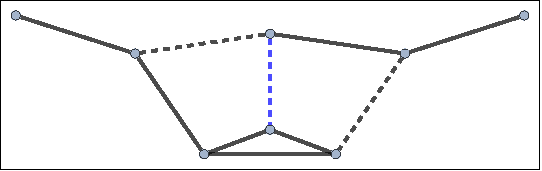
\includegraphics[width=0.6\linewidth]{img/0wyc1k9e4tb0q.pdf}
\end{figure}
\FloatBarrier

\begin{Shaded}
\begin{Highlighting}[]
\NormalTok{FCGraphCuttableQ}\OperatorTok{[}\NormalTok{graph2}\OperatorTok{,} \OperatorTok{\{}\NormalTok{m1}\OperatorTok{\}]}
\end{Highlighting}
\end{Shaded}

\begin{dmath*}\breakingcomma
\text{True}
\end{dmath*}

In the case of graphs with more than 2 external legs, the situation is
somewhat more involved

\begin{Shaded}
\begin{Highlighting}[]
\NormalTok{graph3 }\ExtensionTok{=} \OperatorTok{\{\{}\SpecialCharTok{{-}}\DecValTok{4} \OtherTok{{-}\textgreater{}} \DecValTok{4}\OperatorTok{,} \SpecialCharTok{{-}}\DecValTok{3} \OtherTok{{-}\textgreater{}} \DecValTok{1}\OperatorTok{,} \SpecialCharTok{{-}}\DecValTok{2} \OtherTok{{-}\textgreater{}} \DecValTok{2}\OperatorTok{,} \SpecialCharTok{{-}}\DecValTok{1} \OtherTok{{-}\textgreater{}} \DecValTok{3}\OperatorTok{,} \DecValTok{1} \OtherTok{{-}\textgreater{}} \DecValTok{4}\OperatorTok{,} \DecValTok{1} \OtherTok{{-}\textgreater{}} \DecValTok{6}\OperatorTok{,} \DecValTok{2} \OtherTok{{-}\textgreater{}} \DecValTok{3}\OperatorTok{,} \DecValTok{2} \OtherTok{{-}\textgreater{}} \DecValTok{6}\OperatorTok{,} \DecValTok{3} \OtherTok{{-}\textgreater{}} \DecValTok{5}\OperatorTok{,} \DecValTok{4} \OtherTok{{-}\textgreater{}} \DecValTok{5}\OperatorTok{,} \DecValTok{5} \OtherTok{{-}\textgreater{}} \DecValTok{6}\OperatorTok{\},} 
   \OperatorTok{\{}\NormalTok{Q1 }\SpecialCharTok{{-}}\NormalTok{ Q2 }\SpecialCharTok{{-}}\NormalTok{ Q3}\OperatorTok{,}\NormalTok{ Q1}\OperatorTok{,}\NormalTok{ Q2}\OperatorTok{,}\NormalTok{ Q3}\OperatorTok{,} \OperatorTok{\{}\SpecialCharTok{{-}}\NormalTok{p1 }\SpecialCharTok{{-}}\NormalTok{ p2 }\SpecialCharTok{+}\NormalTok{ Q2 }\SpecialCharTok{+}\NormalTok{ Q3}\OperatorTok{,} \DecValTok{1}\OperatorTok{,} \DecValTok{0}\OperatorTok{\},} \OperatorTok{\{}\SpecialCharTok{{-}}\NormalTok{p1 }\SpecialCharTok{{-}}\NormalTok{ p2 }\SpecialCharTok{+}\NormalTok{ Q2}\OperatorTok{,} \DecValTok{1}\OperatorTok{,} \DecValTok{0}\OperatorTok{\},} \OperatorTok{\{}\NormalTok{p1}\OperatorTok{,} \DecValTok{1}\OperatorTok{,} \SpecialCharTok{{-}}\NormalTok{m1}\SpecialCharTok{\^{}}\DecValTok{2}\OperatorTok{\},} \OperatorTok{\{}\SpecialCharTok{{-}}\NormalTok{p1 }\SpecialCharTok{+}\NormalTok{ Q2}\OperatorTok{,} \DecValTok{1}\OperatorTok{,} \DecValTok{0}\OperatorTok{\},} 
     \OperatorTok{\{}\NormalTok{p1 }\SpecialCharTok{+}\NormalTok{ Q1}\OperatorTok{,} \DecValTok{1}\OperatorTok{,} \SpecialCharTok{{-}}\NormalTok{m3}\SpecialCharTok{\^{}}\DecValTok{2}\OperatorTok{\},} \OperatorTok{\{}\NormalTok{p1 }\SpecialCharTok{+}\NormalTok{ p2 }\SpecialCharTok{+}\NormalTok{ Q1}\OperatorTok{,} \DecValTok{1}\OperatorTok{,} \DecValTok{0}\OperatorTok{\},} \OperatorTok{\{}\NormalTok{p2}\OperatorTok{,} \DecValTok{1}\OperatorTok{,} \SpecialCharTok{{-}}\NormalTok{m2}\SpecialCharTok{\^{}}\DecValTok{2}\OperatorTok{\}\},} \OperatorTok{\{}\DecValTok{0}\OperatorTok{,} \DecValTok{0}\OperatorTok{,} \DecValTok{0}\OperatorTok{,} \DecValTok{0}\OperatorTok{,}\NormalTok{ SFAD}\OperatorTok{[\{\{}\NormalTok{p1 }\SpecialCharTok{+}\NormalTok{ p2 }\SpecialCharTok{+}\NormalTok{ Q1}\OperatorTok{,} \DecValTok{0}\OperatorTok{\},} \OperatorTok{\{}\DecValTok{0}\OperatorTok{,} \DecValTok{1}\OperatorTok{\},} \DecValTok{1}\OperatorTok{\}],} 
\NormalTok{     SFAD}\OperatorTok{[\{\{}\SpecialCharTok{{-}}\NormalTok{p1 }\SpecialCharTok{+}\NormalTok{ Q2}\OperatorTok{,} \DecValTok{0}\OperatorTok{\},} \OperatorTok{\{}\DecValTok{0}\OperatorTok{,} \DecValTok{1}\OperatorTok{\},} \DecValTok{1}\OperatorTok{\}],}\NormalTok{ SFAD}\OperatorTok{[\{\{}\NormalTok{p2}\OperatorTok{,} \DecValTok{0}\OperatorTok{\},} \OperatorTok{\{}\NormalTok{m2}\SpecialCharTok{\^{}}\DecValTok{2}\OperatorTok{,} \DecValTok{1}\OperatorTok{\},} \DecValTok{1}\OperatorTok{\}],}\NormalTok{ SFAD}\OperatorTok{[\{\{}\NormalTok{p1}\OperatorTok{,} \DecValTok{0}\OperatorTok{\},} \OperatorTok{\{}\NormalTok{m1}\SpecialCharTok{\^{}}\DecValTok{2}\OperatorTok{,} \DecValTok{1}\OperatorTok{\},} \DecValTok{1}\OperatorTok{\}],} 
\NormalTok{     SFAD}\OperatorTok{[\{\{}\NormalTok{p1 }\SpecialCharTok{+}\NormalTok{ Q1}\OperatorTok{,} \DecValTok{0}\OperatorTok{\},} \OperatorTok{\{}\NormalTok{m3}\SpecialCharTok{\^{}}\DecValTok{2}\OperatorTok{,} \DecValTok{1}\OperatorTok{\},} \DecValTok{1}\OperatorTok{\}],}\NormalTok{ SFAD}\OperatorTok{[\{\{}\SpecialCharTok{{-}}\NormalTok{p1 }\SpecialCharTok{{-}}\NormalTok{ p2 }\SpecialCharTok{+}\NormalTok{ Q2}\OperatorTok{,} \DecValTok{0}\OperatorTok{\},} \OperatorTok{\{}\DecValTok{0}\OperatorTok{,} \DecValTok{1}\OperatorTok{\},} \DecValTok{1}\OperatorTok{\}],} 
\NormalTok{     SFAD}\OperatorTok{[\{\{}\SpecialCharTok{{-}}\NormalTok{p1 }\SpecialCharTok{{-}}\NormalTok{ p2 }\SpecialCharTok{+}\NormalTok{ Q2 }\SpecialCharTok{+}\NormalTok{ Q3}\OperatorTok{,} \DecValTok{0}\OperatorTok{\},} \OperatorTok{\{}\DecValTok{0}\OperatorTok{,} \DecValTok{1}\OperatorTok{\},} \DecValTok{1}\OperatorTok{\}]\},} \DecValTok{1}\OperatorTok{\}}
\end{Highlighting}
\end{Shaded}

\begin{dmath*}\breakingcomma
\left\{\{-4\to 4,-3\to 1,-2\to 2,-1\to 3,1\to 4,1\to 6,2\to 3,2\to 6,3\to 5,4\to 5,5\to 6\},\left\{\text{Q1}-\text{Q2}-\text{Q3},\text{Q1},\text{Q2},\text{Q3},\{-\text{p1}-\text{p2}+\text{Q2}+\text{Q3},1,0\},\{-\text{p1}-\text{p2}+\text{Q2},1,0\},\left\{\text{p1},1,-\text{m1}^2\right\},\{\text{Q2}-\text{p1},1,0\},\left\{\text{p1}+\text{Q1},1,-\text{m3}^2\right\},\{\text{p1}+\text{p2}+\text{Q1},1,0\},\left\{\text{p2},1,-\text{m2}^2\right\}\right\},\left\{0,0,0,0,\frac{1}{((\text{p1}+\text{p2}+\text{Q1})^2+i \eta )},\frac{1}{((\text{Q2}-\text{p1})^2+i \eta )},\frac{1}{(\text{p2}^2-\text{m2}^2+i \eta )},\frac{1}{(\text{p1}^2-\text{m1}^2+i \eta )},\frac{1}{((\text{p1}+\text{Q1})^2-\text{m3}^2+i \eta )},\frac{1}{((-\text{p1}-\text{p2}+\text{Q2})^2+i \eta )},\frac{1}{((-\text{p1}-\text{p2}+\text{Q2}+\text{Q3})^2+i \eta )}\right\},1\right\}
\end{dmath*}

\begin{Shaded}
\begin{Highlighting}[]
\NormalTok{FCLoopGraphPlot}\OperatorTok{[}\NormalTok{graph3}\OperatorTok{,} \FunctionTok{GraphPlot} \OtherTok{{-}\textgreater{}} \OperatorTok{\{}\FunctionTok{MultiedgeStyle} \OtherTok{{-}\textgreater{}} \FloatTok{0.35}\OperatorTok{,} \FunctionTok{Frame} \OtherTok{{-}\textgreater{}} \ConstantTok{True}\OperatorTok{,} \FunctionTok{VertexLabels} \OtherTok{{-}\textgreater{}} \StringTok{"Name"}\OperatorTok{\},} \FunctionTok{Style} \OtherTok{{-}\textgreater{}} \OperatorTok{\{}
       \OperatorTok{\{}\StringTok{"InternalLine"}\OperatorTok{,}\NormalTok{ \_}\OperatorTok{,}\NormalTok{ \_}\OperatorTok{,} \AttributeTok{mm\_} \SpecialCharTok{/}\NormalTok{; ! }\FunctionTok{FreeQ}\OperatorTok{[}\NormalTok{mm}\OperatorTok{,}\NormalTok{ m1}\OperatorTok{]\}} \OtherTok{{-}\textgreater{}} \OperatorTok{\{}\FunctionTok{Red}\OperatorTok{,} \FunctionTok{Thick}\OperatorTok{\},} 
       \OperatorTok{\{}\StringTok{"InternalLine"}\OperatorTok{,}\NormalTok{ \_}\OperatorTok{,}\NormalTok{ \_}\OperatorTok{,} \AttributeTok{mm\_} \SpecialCharTok{/}\NormalTok{; ! }\FunctionTok{FreeQ}\OperatorTok{[}\NormalTok{mm}\OperatorTok{,}\NormalTok{ m2}\OperatorTok{]\}} \OtherTok{{-}\textgreater{}} \OperatorTok{\{}\FunctionTok{Blue}\OperatorTok{,} \FunctionTok{Thick}\OperatorTok{\},} 
       \OperatorTok{\{}\StringTok{"InternalLine"}\OperatorTok{,}\NormalTok{ \_}\OperatorTok{,}\NormalTok{ \_}\OperatorTok{,} \AttributeTok{mm\_} \SpecialCharTok{/}\NormalTok{; ! }\FunctionTok{FreeQ}\OperatorTok{[}\NormalTok{mm}\OperatorTok{,}\NormalTok{ m3}\OperatorTok{]\}} \OtherTok{{-}\textgreater{}} \OperatorTok{\{}\FunctionTok{Green}\OperatorTok{,} \FunctionTok{Thick}\OperatorTok{\},} 
       \OperatorTok{\{}\StringTok{"InternalLine"}\OperatorTok{,}\NormalTok{ \_}\OperatorTok{,}\NormalTok{ \_}\OperatorTok{,} \AttributeTok{mm\_} \SpecialCharTok{/}\NormalTok{; ! }\FunctionTok{FreeQ}\OperatorTok{[}\NormalTok{mm}\OperatorTok{,}\NormalTok{ m4}\OperatorTok{]\}} \OtherTok{{-}\textgreater{}} \OperatorTok{\{}\FunctionTok{Purple}\OperatorTok{,} \FunctionTok{Thick}\OperatorTok{\},} 
       \OperatorTok{\{}\StringTok{"ExternalLine"}\OperatorTok{,}\NormalTok{ q1}\OperatorTok{\}} \OtherTok{{-}\textgreater{}} \OperatorTok{\{}\FunctionTok{Brown}\OperatorTok{,} \FunctionTok{Thick}\OperatorTok{,} \FunctionTok{Dashed}\OperatorTok{\}} 
      \OperatorTok{\}]}
\end{Highlighting}
\end{Shaded}

\FloatBarrier
\begin{figure}[!ht]
\centering
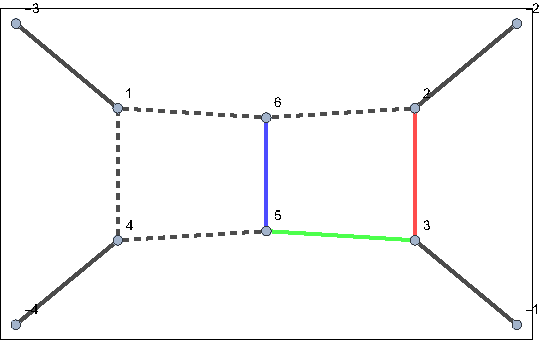
\includegraphics[width=0.6\linewidth]{img/0vqfnrsj37rjh.pdf}
\end{figure}
\FloatBarrier

By default \texttt{FCGraphCuttableQ} thinks that the graph is not
cuttable, since it choses the path connecting two external edges on the
same side

\begin{Shaded}
\begin{Highlighting}[]
\NormalTok{FCGraphCuttableQ}\OperatorTok{[}\NormalTok{graph3}\OperatorTok{,} \OperatorTok{\{}\NormalTok{m1}\OperatorTok{,}\NormalTok{ m2}\OperatorTok{,}\NormalTok{ m3}\OperatorTok{\}]}
\end{Highlighting}
\end{Shaded}

\begin{dmath*}\breakingcomma
\text{False}
\end{dmath*}

\begin{Shaded}
\begin{Highlighting}[]
\NormalTok{FCGraphFindPath}\OperatorTok{[}\NormalTok{graph3}\OperatorTok{[[}\DecValTok{1}\OperatorTok{]],} \OperatorTok{\{}\DecValTok{1}\OperatorTok{,} \DecValTok{1}\OperatorTok{,} \DecValTok{1}\OperatorTok{,} \DecValTok{1}\OperatorTok{,} \SpecialCharTok{{-}}\DecValTok{1}\OperatorTok{,} \SpecialCharTok{{-}}\DecValTok{1}\OperatorTok{,} \DecValTok{1}\OperatorTok{,} \SpecialCharTok{{-}}\DecValTok{1}\OperatorTok{,} \DecValTok{1}\OperatorTok{,} \SpecialCharTok{{-}}\DecValTok{1}\OperatorTok{,} \DecValTok{1}\OperatorTok{\}]}
\end{Highlighting}
\end{Shaded}

\begin{dmath*}\breakingcomma
\left(
\begin{array}{ccc}
 \{-2\to 2,3\} & \{2\to 3,7\} & \{-1\to 3,4\} \\
\end{array}
\right)
\end{dmath*}

We can exclude such paths by letting the function know which external
edges are on the same side via the option
\texttt{SameSideExternalEdges}. In this case \texttt{FCGraphCuttableQ}
correctly reports that the graph is cuttable

\begin{Shaded}
\begin{Highlighting}[]
\NormalTok{FCGraphCuttableQ}\OperatorTok{[}\NormalTok{graph3}\OperatorTok{,} \OperatorTok{\{}\NormalTok{m1}\OperatorTok{,}\NormalTok{ m2}\OperatorTok{,}\NormalTok{ m3}\OperatorTok{\},}\NormalTok{ SameSideExternalEdges }\OtherTok{{-}\textgreater{}} \OperatorTok{\{}\SpecialCharTok{{-}}\DecValTok{2}\OperatorTok{,} \SpecialCharTok{{-}}\DecValTok{1}\OperatorTok{\}]}
\end{Highlighting}
\end{Shaded}

\begin{dmath*}\breakingcomma
\text{True}
\end{dmath*}
\end{document}
